\usetikzlibrary{decorations.markings}
\newif\iflabrev

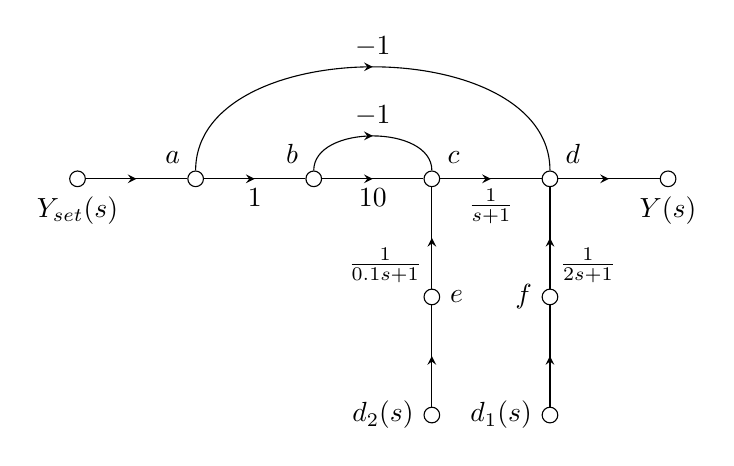
\begin{tikzpicture}
[
label revd/.is if=labrev,
%label revd/.default=true,
amark/.style={
            decoration={             
                        markings,   
                        mark=at position {0.5} with { 
                                    \arrow{stealth},
                                    \iflabrev \node[above] {#1};\else \node[below] {#1};\fi
                        }
            },
            postaction={decorate}
},
terminal/.style 2 args={draw,circle,inner sep=2pt,label={#1:#2}},
]

%Place the nodes
\node[terminal={below}{$Y_{set}(s)$}] (ysp) at (0,0) {};
\node[terminal={above left}{$a$}] (a) at (1.5,0) {};
\node[terminal={above left}{$b$}] (b) at (3,0) {};
\node[terminal={above right}{$c$}] (c) at (4.5,0) {};
\node[terminal={above right}{$d$}] (d) at (6,0) {};
\node[terminal={right}{$e$}] (e) at (4.5,-1.5) {};
\node[terminal={left}{$f$}] (f) at (6,-1.5) {};
\node[terminal={below}{$Y(s)$}] (ys) at (7.5,0) {};
\node[terminal={left}{$d_2(s)$}] (d2s) at (4.5,-3) {};
\node[terminal={left}{$d_1(s)$}] (d1s) at (6,-3) {};

%Draw the connections
\draw[amark](ysp) to (a);
\draw[amark=$1$] (a) to (b);
\draw[amark=$10$] (b) to (c);
\draw[amark=$-1$,label revd] (b) to[bend left=90] (c);
\draw[amark=$\frac{1}{s+1}$] (c) to (d);
\draw[amark] (d) to (ys);
\draw[amark=$-1$,label revd] (a) to[bend left=90] (d);
\draw[amark] (e) to node[midway, below left] {$\frac{1}{0.1s+1}$} (c);
\draw[amark] (f) to node[midway, below right] {$\frac{1}{2s+1}$} (d);
\draw[amark](d2s) to (e);
\draw[amark](d1s) to (f);
\end{tikzpicture}
